%%%%%%%%%%%%%%%%%%%%%%%%%%%%%%%%%%%%%%%%%%%%%%%%%%%%%%%%%%%%%%%%%%%%%%%%%%%%%%%
% Copyright 2020
% Little Compline with Akathist to the Theotokos
% as  served on the first 4 Fridays of Great Lent
%%%%%%%%%%%%%%%%%%%%%%%%%%%%%%%%%%%%%%%%%%%%%%%%%%%%%%%%%%%%%%%%%%%%%%%%%%%%%%%

\documentclass[twoside, letterpaper, 12pt]{report}
\usepackage{orthodoxservicebook}
\usepackage{litanies}

\title{Divine Liturgy of the Presanctified Gifts\\
       Celebrated on Weekdays of Great Lent}
\date{}% Remove date
\author{}
\titlepic{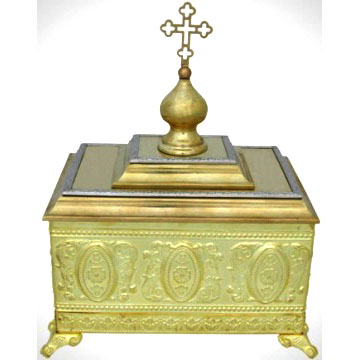
\includegraphics[width=0.5\textwidth]{tabernacle-2.jpg}}

\begin{document}
\maketitle
\pagestyle{empty} % Don't show page numbers

\instruction{This page intentionally left blank}

\cleardoublepage
\pagestyle{plain}
\setcounter{page}{1}

\chapter*{Lenten Liturgy of the Presanctified Gifts}

\deaconline{Bless, Master!}
\priestline{\blessedisthekingdom}

\choralresponse{./Z-Responses/RussianPresanctified/Amen.ly}

\peopleline{\comeletusworship}

\centeredsection{Psalm 103}
\begin{maybetwocolumns}
  \input{Psalms/Psalm103.txt}

  \instruction{And again:}

  The sun knoweth his going down. Thou appointedst the darkness, and there was the night.
  How magnified are Thy works, O Lord! In wisdom hast Thou made them all.
\end{maybetwocolumns}

\begin{reader}
  \item \gne
  \item Alleluia, Alleluia, Alleluia. Glory to Thee, O God. \thrice\\
        O our God and our Hope, glory to Thee!
\end{reader}

\begin{priest}
  \item \small{\instruction{(Quietly)} O Lord our God,
    Thou upholdest all things by Thy pure and perfect hand,
    Thou art patient with us all and mournest over our wickedness:
    remember Thy compassions and Thy mercy.
    Visit us with Thy goodness; and grant us to complete the present day,
    avoiding the diverse plots of the evil one; and preserve our lives free from attack,
    through the grace of Thine all-holy Spirit.
    Through the mercy and love toward mankind of Thine only-begotten Son,
    with Whom Thou art blessed, together with Thine all-holy and good and life-giving Spirit:
    now and ever, and unto ages of ages. Amen.}
  \item \small{\instruction{(Quietly)} O great and wonderful God,
    with Thine inexpressible wisdom, and Thine abundant providence Thou administerest all things.
    Thou hast bestowed on us good things on earth;
    Thou hast given us a pledge of the promised kingdom through the good things
    already bestowed on us;
    and Thou hast made us to flee from all evil during that part of this day which is past:
    Grant us also to complete this day without blame before Thy holy glory, and to glorify Thee,
    our God, Who art the only good One, and Lover of mankind.
    For Thou art our God, and unto Thee we ascribe glory:
    to the Father, and to the Son, and to the Holy Spirit:
    now and ever, and unto ages of ages. Amen.}
  \item \small{\instruction{(Quietly)} O great and most high God,
    Thou alone hast immortality and dwellest in unapproachable light.
    Thou hast made all creation in wisdom. Thou hast separated the light from
    the darkness. Thou hast made the sun to rule the day, the moon and the stars to rule the night.
    Thou hast made us sinners at this present hour worthy to come before Thy face with thanksgiving
    and to offer to Thee our evening praises. Do Thou Thyself, O Lord, Lover of mankind,
    direct our prayer as incense before Thee, and accept it as a fragrant offering.
    Grant us to pass the present evening and the coming night in peace.
    Clothe us with the armor of light.
    Deliver us from the terror of the night and from the pestilence that stalks in the darkness.
    Grant us sleep, which Thou hast appointed for the alleviation of our weakness,
    free from every imagination of the devil. Yea, O Master of all,
    Bestower of good things, may we, being moved toward repentance on our beds, remember Thy
    Name in the night, that, illuminated by meditation on Thy commandments, we may rise up in
    joyfulness of soul to glorify Thy goodness, offering up prayers,
    and supplications to Thy tender love for our sins and for those of all Thy people,
    whom Thou visitest in mercy, through the intercessions of the holy Theotokos.
    For Thou art a good God and lovest mankind, and unto thee
    we ascribe glory: to the Father, and to the Son, and to the Holy Spirit,
    now and ever and unto ages of ages. Amen.}
\end{priest}

\centeredsection{The Great Ektenia}
\thegreatlitany{
  \choralresponse{./Z-Responses/RussianPresanctified/LordHaveMercy.ly}}{
  }{
  }{
  }{
  }{
  \lilypondfile[staffsize=16]{./Z-Responses/RussianPresanctified/MostHolyTheotokosSaveUs.ly}}{
  \choralresponse{Z-Responses/RussianPresanctified/ToTheeOLord.ly}}{
  \choralresponse{Z-Responses/RussianPresanctified/Amen.ly}}

\centeredsection{The Eighteenth Kathisma (First Third)}
\begin{maybetwocolumns}
  \centeredsubsection{Psalm 119}
  \input{./Psalms/Psalm119.txt}
  \centeredsubsection{Psalm 120}
  \input{./Psalms/Psalm120.txt}
  \centeredsection{Psalm 121}
  \input{./Psalms/Psalm121.txt}
  \centeredsection{Psalm 122}
  \input{./Psalms/Psalm122.txt}
  \centeredsection{Psalm 123}
  \input{./Psalms/Psalm123.txt}
\end{maybetwocolumns}

\begin{reader}
  \item \gne
  \item \alleluiathriceglorytotheethrice
  \item \glory
\end{reader}

\centeredsection{The Little Litany}
\thelittlelitany{
  \choralresponse{./Z-Responses/RussianPresanctified/LordHaveMercy.ly}}{
  \choralresponse{./Z-Responses/RussianPresanctified/LordHaveMercy.ly}}{
  \lilypondfile[staffsize=16]{./Z-Responses/RussianPresanctified/MostHolyTheotokosSaveUs.ly}}{
  \choralresponse{./Z-Responses/RussianPresanctified/Amen.ly}}

\readerline{\nowandever}

\centeredsection{The Eighteenth Kathisma (Second Third)}
\begin{maybetwocolumns}
  \centeredsubsection{Psalm 124}
  \input{./Psalms/Psalm124.txt}
  \centeredsubsection{Psalm 125}
  \input{./Psalms/Psalm125.txt}
  \centeredsection{Psalm 126}
  \input{./Psalms/Psalm126.txt}
  \centeredsection{Psalm 127}
  \input{./Psalms/Psalm127.txt}
  \centeredsection{Psalm 128}
  \input{./Psalms/Psalm128.txt}
\end{maybetwocolumns}

\begin{reader}
  \item \gne
  \item \alleluiathriceglorytotheethrice
  \item \glory
\end{reader}

\centeredsection{The Little Litany}
\thelittlelitany{
  \choralresponse{./Z-Responses/RussianPresanctified/LordHaveMercy.ly}}{
  \choralresponse{./Z-Responses/RussianPresanctified/LordHaveMercy.ly}}{
  \lilypondfile[staffsize=16]{./Z-Responses/RussianPresanctified/MostHolyTheotokosSaveUs.ly}}{
  \choralresponse{./Z-Responses/RussianPresanctified/Amen.ly}}

\centeredsection{The Eighteenth Kathisma (Last Third)}
\begin{maybetwocolumns}
  \centeredsubsection{Psalm 129}
  \input{./Psalms/Psalm129.txt}
  \centeredsubsection{Psalm 130}
  \input{./Psalms/Psalm130.txt}
  \centeredsection{Psalm 131 First Part}
  \input{./Psalms/Psalm131-pt1.txt}

  \instruction{The reader stops and all kneel until the priest finishes censing the lamb 3 times.   }

  \centeredsection{Psalm 131 Continued}
  \input{./Psalms/Psalm131-pt2.txt}
  \centeredsection{Psalm 132}
  \input{./Psalms/Psalm132.txt}
  \centeredsection{Psalm 133}
  \input{./Psalms/Psalm133.txt}
\end{maybetwocolumns}

\begin{reader}
  \item \gne
  \item \alleluiathriceglorytotheethrice
  \item \oourgodandourhopeglorytothee
\end{reader}

\instruction{The priest says several prayers here quietly.}

\centeredsection{The Little Litany}
\thelittlelitany{
  \choralresponse{./Z-Responses/RussianPresanctified/LordHaveMercy.ly}}{
  \choralresponse{./Z-Responses/RussianPresanctified/LordHaveMercy.ly}}{
  \lilypondfile[staffsize=16]{./Z-Responses/RussianPresanctified/MostHolyTheotokosSaveUs.ly}}{
  \choralresponse{./Z-Responses/RussianPresanctified/Amen.ly}}

\centeredsection{O Lord I Have Cried}
\instruction{Chanted in the tone as prescribed}

\centeredsection{The Holy Entrance}
\instruction{If the Entrance is made with the Gospel Book,
the Deacon replaces the orarion over the Gospel while the Priest blesses the Entrance.
The Deacon offers the Gospel Book for veneration by the Priest, himself kissing the Priest’s right hand.
The Deacon turns and faces the Holy Altar and elevates the Gospel Book.}

\deaconline{Wisdom! Let us attend!}

\centeredsection{O Gladsome Light}
\lilypondfile{./1-Vespers/Gladsome_Light/JoyousLightByz-Music.ly}

\centeredsection{Old Testament Passages}
\instruction{As prescribed for the week}

\centeredsection{Let My Prayer Arise}

\begin{priest}
  \item Let my prayer arise in Thy sight as incense;
    and let the lifting up of my hands be an evening sacrifice.
  \item Lord, I have cried out unto Thee, hear me;
    attend to the voice of my supplication when I cry unto Thee.
\end{priest}

\peopleline{\instruction{Repeat the following refrain after each verse said by the priest}}

\lilypondfile{./Triodion/LetMyPrayerArise/LetMyPrayerArise-Arabic-Music.ly}

\begin{priest}
  \item Set a watch, O Lord, before my mouth, and a protecting door round about my lips.
  \item Incline not my heart to evil words, to make excuses in sins.
  \item \glory
  \item \nowandever
\end{priest}

\priestline{\instruction{The Priest, still in front of the Holy Table,
  censes as he begins chanting the following verse.
  at 'In Thy Sight..' the priest turns to stand at the Holy Doors and censes the Icon of Christ on
  the iconostasis as he continues.}}
\choralresponse{./Triodion/LetMyPrayerArise/LetMyPrayerArise-Arabic-EndPt1-Music.ly}

\peopleline{\instruction{The choir concludes:}}
\choralresponse{./Triodion/LetMyPrayerArise/LetMyPrayerArise-Arabic-EndPt2-Music.ly}

\end{document}